\chapter{研究方法}
\label{cha:method}

\section{研究方法概述}
本文提出的研究方法分为两个主要部分:离线工作算法和运行时工作算法(如图\ref{fig:stepMap})。
%\begin{wrapfigure}{r}{1.0\linewidth}
%	\centering
%	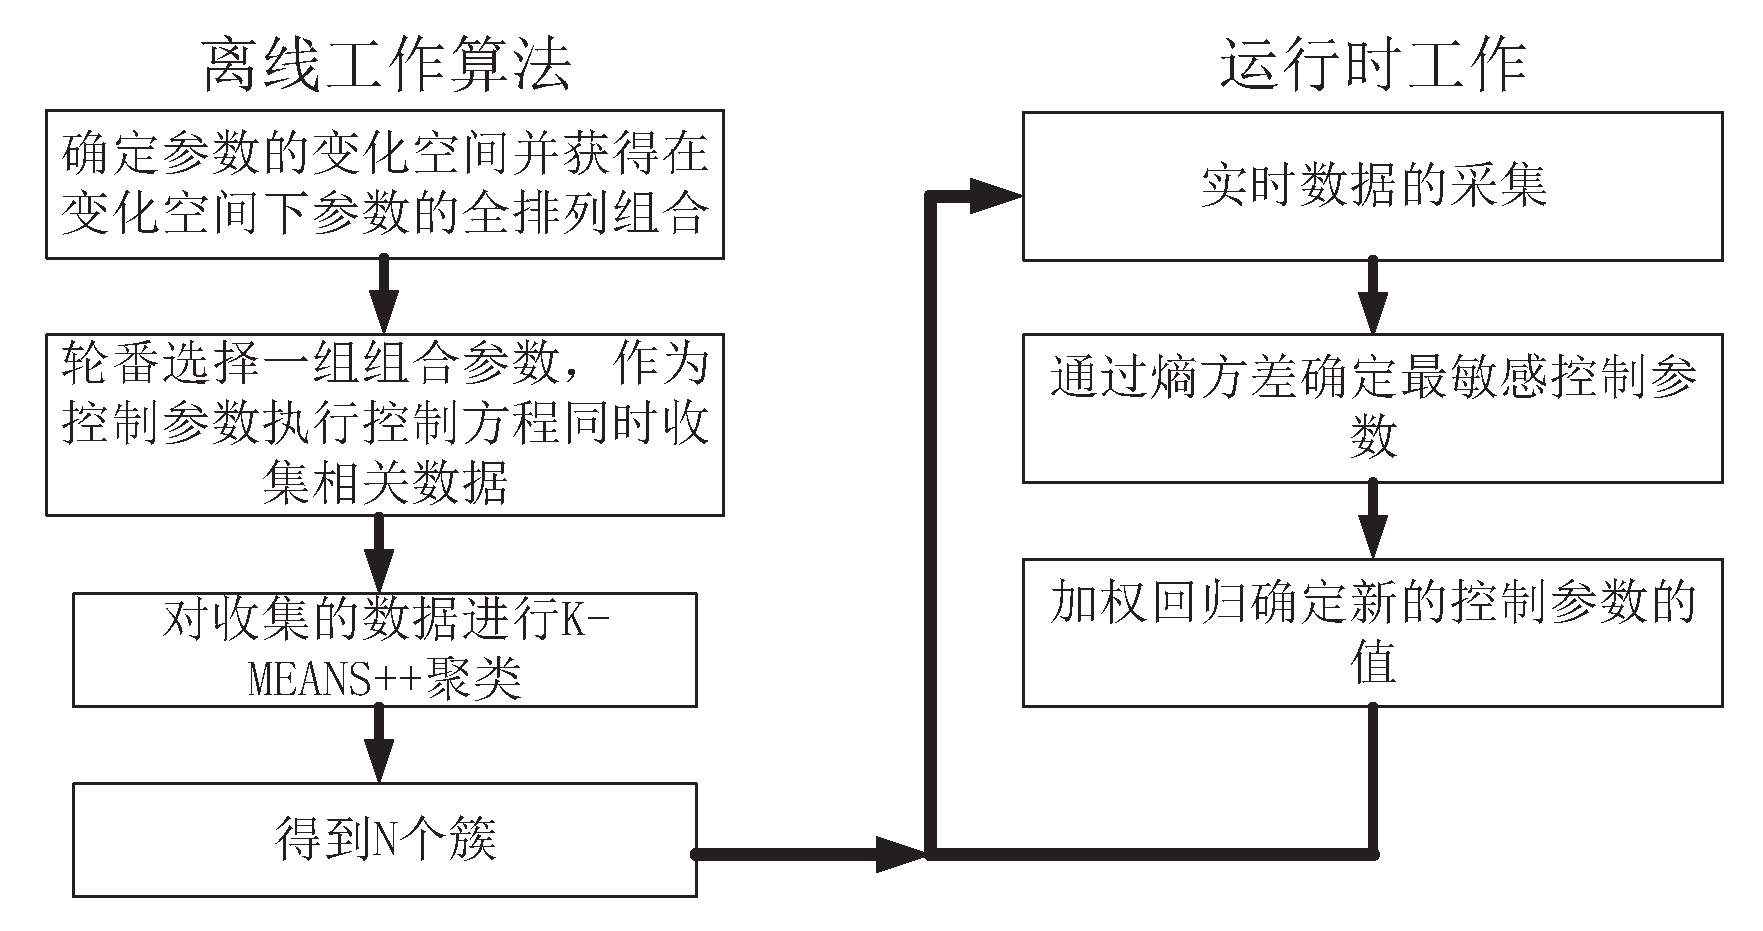
\includegraphics[width=0.8\textwidth]{figure/chap03/step.eps}
%	\caption{研究方法概述}
%	\label{fig:stepMap}
%\end{wrapfigure}
\begin{figure}[h]
	\centering
	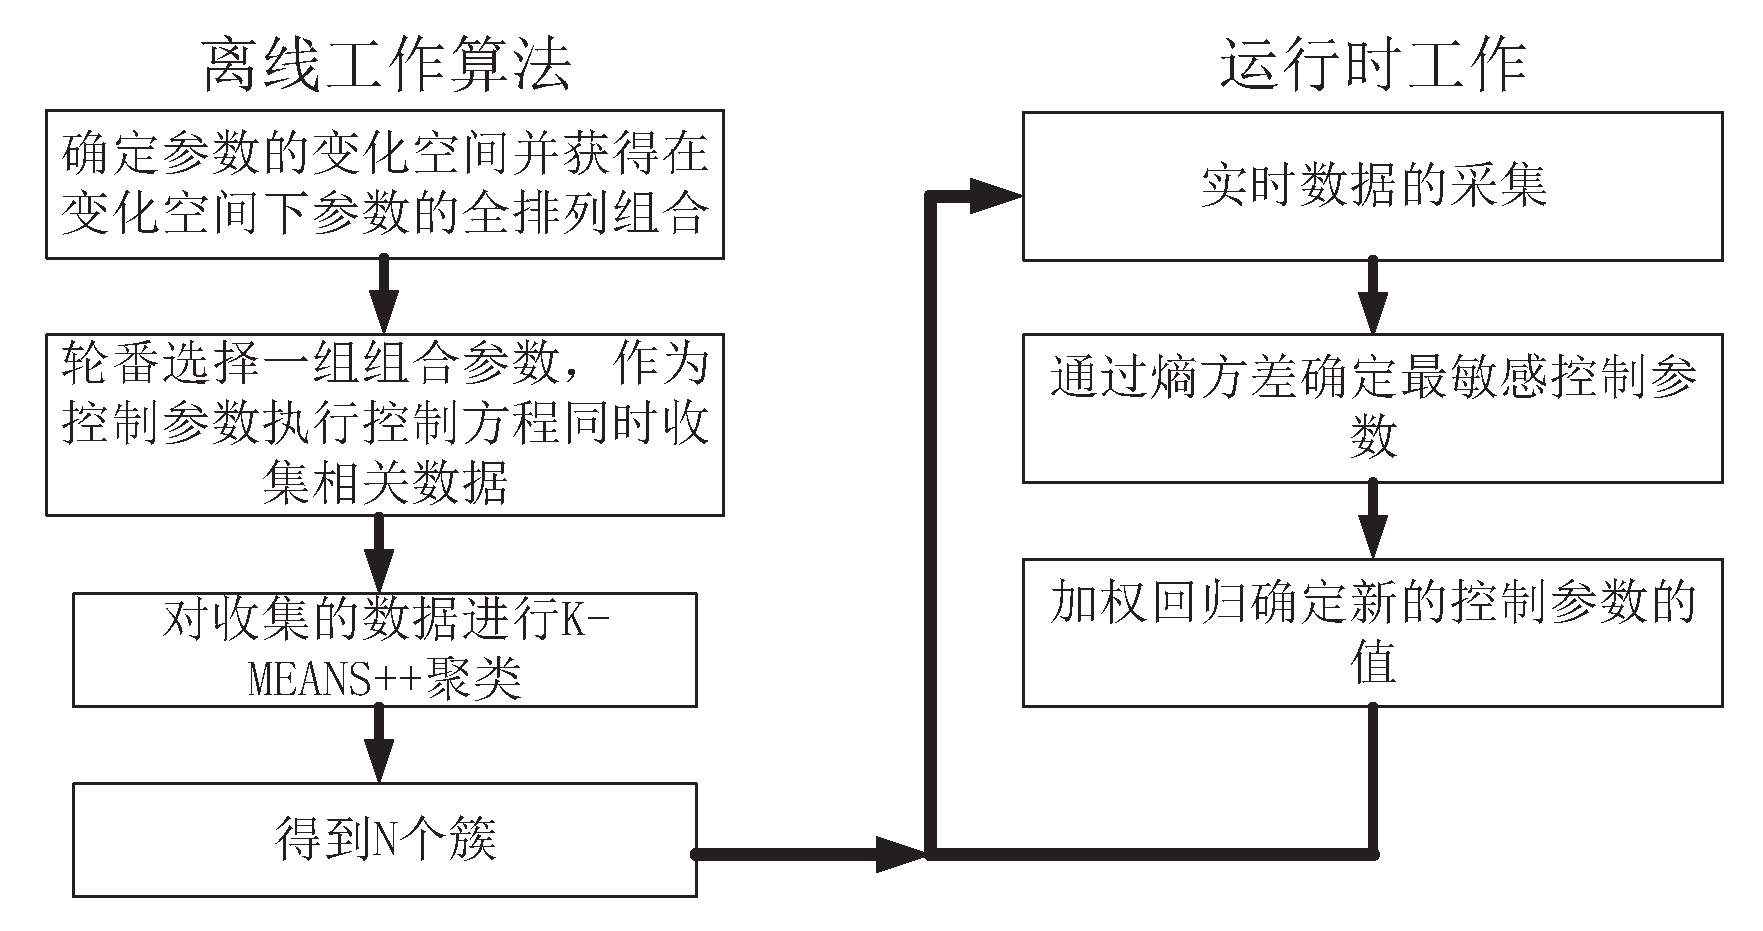
\includegraphics[width=0.8\textwidth]{figure/chap03/step.eps}
	\caption{研究方法概述}
	\label{fig:stepMap}
\end{figure}

在离线工作算法中,第一步,先定义控制参数的变化空间,让机器人在不同的参数组合的控制方程下爬杆,在爬杆过程中控制方程中的参数是不变的。当机器人爬杆时,以2秒为周期记录机器人的Z轴方向加速度以及关节角度。最后,将在所有参数组合控制下的蛇形机器人爬杆运动中采集到的数据全部整合成一个大数据集,然后对整个数据集采取K-MEANS++算法实现聚类~\cite{Cluseter_ICT}~\cite{KmeansAndDeepLearning}。

在运行时工作算法中,首先给定机器人已初始化好的控制参数。在机器人爬杆过程中,以2秒为周期收集机器人实时的关节角度,加速度和当前控制参数的数据值,然后通过归簇操作在离线工作算法中得到的数据簇中抽取同簇的数据集合。在获取到同簇的数据集合后,通过熵方差计算衡量每个控制参数对机器人运动的影响程度,最终挑取影响程度最大的控制参数,即最敏感控制参数。最终通过加权回归得到最敏感控制参数的新值后代入控制方程从而改变蛇形机器人运动步态。

\section{离线工作算法}
在离线工作算法的预处理工作中,让机器人分别在直径为25\,cm 和 35\,cm的杆上进行大量的尝试性攀爬运动,并且在攀爬过程中收集存储数据,存储数据类型如表\,\ref{dataTable}所示。

\begin{table}[h]
	\begin{center}
		\caption{机器人训练时记录的数据类型}
		\label{dataTable}
		\begin{tabular}{cl cl} 
			\toprule
			\multicolumn{1}{m{3cm}}{\centering 数据类型}
			&\multicolumn{1}{m{4cm}}
			{\centering Definition}\\
			\midrule
			\multirow{2}{*}{$\theta_{m,i}$} & \multirow{2}{*}{第i个关节的关节角度值} \\
			\multirow{2}{*}{$M$} & \multirow{2}{*}{所测量的所有关节角角度的均值} \\
			\multirow{2}{*}{$a_{z}$} & \multirow{2}{*}{Z轴的加速度值} \\\\	\hline
			\multirow{2}{*}{$A$} & \multirow{2}{*}{幅度(控制参数)的值} \\
			\multirow{2}{*}{$\omega$} & \multirow{2}{*}{角速度(控制参数)的值} \\
			\multirow{2}{*}{$\varepsilon$} & \multirow{2}{*}{相位(控制参数)的值} \\\\
			\bottomrule
		\end{tabular}
	\end{center}
\end{table}

我们定义$M=$$\frac{\sum_{i=1}^{n}\theta_{m,i}}{n}$其中,n是关节总数量。$\theta_{m}=\begin{bmatrix}\theta_{m,1} & \theta_{m,2} & \cdots & \theta_{m,n}\end{bmatrix}$是测量得到的关节角度值集合。控制参数矢量为$\begin{bmatrix}A& \omega&\varepsilon\end{bmatrix}$,其中$A$是幅度参数, $\omega$是角速度参数,$\varepsilon$是相位参数(式(\ref{basicRoll}))。

在收集完蛇形机器人的训练数据之后,我们将蛇形机器人在两个不同直径的杆上训练得到的数据合并成一个大数据集,然后对数据做聚类,目的是为了在运行时工作算法中对计算性能进行优化。

在本文中,训练过程即离线工作算法中收集到的数据是一个大数据集。由于K-MEANS++算法在大数据集下工作具有效率高和可拓展性的优点,因此我们采用K-MEANS++算法执行聚类操作。将训练集最终聚类出$N$个簇。聚类过程可以分为如下几个步骤:

\begin{itemize}
	\item 步骤 1:通过方程\ref{clu_var}确定 $N$ 的值。
	\begin{eqnarray}\label{clu_var}
	N=arg\min \limits_{N_{k}}{\frac{\sum _{N_{k}}(S_{i}-E)^{2}}{N_{k}}}
	\end{eqnarray}
	其中 $E = \frac{\sum _{N}(S_{i})}{N_{k}}$,$i\in [1,N_{k}]$。$S_{i}$是每个簇中成员数据到簇心的距离的均值。
	\item 步骤 2:执行 K-MEANS++ 算法,伪代码如算法\ref{KMEANS++}所示。K-MEANS++ 是K-MEANS算法的改进版本。通过初始化函数INITILIZE,我们可以得到 $N$ 个初始化的簇心。然后, 我们迭代运行更新函数UPDATE来不断更新簇心和数据在$N$个簇中的归属直到簇心在误差范围内不再变化为止。
\end{itemize}

\begin{algorithm}[h]
	\KwIn{训练数据集$\mybold{P}$,簇的数量$N$}
	\KwOut{簇心的数据集$\mybold{X}$}
	FUNCTION INITIALIZATION($\mybold{P}$,$N$) \Begin{
		$\mybold{X}$ $\gets$ 从$\mybold{P}$中随机选取一个数据矢量\\
		\While{$\vert \mybold{X} \vert < N$}{
			\For{$i = 1 \to \vert \mybold{P} \vert$}{
				$I \gets arg\min \limits_{i}\left({\sum_{j=1}^{\vert \mybold{X} \vert} {\Vert X_j - P_i \Vert}^2  }\right)$ \\
				$\mybold{X} \gets \mybold{X} \cup \left\{ P_I \right\}$\\
				$\mybold{P} \gets \mybold{P} - P_I$
			}
		}
		\Return{$\mybold{X}$}
	}
	FUNCTION UPDATE($\mybold{P}$,$\mybold{X}$) \Begin{
		\While{$\mybold{X}$在误差范围内不再变化}{
			\For{$i = 1 \to \vert \mybold{P} \vert$}{
				$C_i \gets arg\min \limits_{k}{\left( {\Vert P_i - X_k\Vert} ^2\right)}$
			}
			\For{$k = 1 \to \vert \mybold{X} \vert$}{
				$X_k \gets \frac{\sum_{i}{\left\{C_i=k\right\}P_i}}{\sum_{i}{\left\{C_i=k\right\}}}$
			}
		}
		\Return{$\mybold{X}$}
	}
	
	\caption{K-MEANS++算法}
	\label{KMEANS++}
\end{algorithm}

通过使用K-MEANS++算法对训练数据集$\mybold{P}$进行聚类,$\mybold{P}$可以被分类成$N$个簇。聚类算法输出的数据格式为两个部分:
\begin{enumerate}
	\item 簇心数据集$\mybold{X}$.
	\item 属于簇心 $X_{k}(k \in [1,N]$)的簇的数据$P_{i}(i \in [1,\vert \mybold{P} \vert]$)
\end{enumerate}

\section{运行时工作算法}

在蛇形机器人实时运行进行爬杆运动时,将周期性地采集实时数据,然后执行运行时工作算法。首先,我们根据离线工作中训练得到的聚类结果对实时采集的数据做归簇操作,然后可以选取同簇中的训练数据,基于这部分数据计算熵方差,选出最敏感的参数,即对步态运动影响最大的步态参数。最后,使用回归分析思想,修改选定的步态参数,保持其他参数不变。

\subsection{基于熵方差的参数选择}
\subsubsection{实时数据的归簇}
每当我们采集到一组实时数据,我们都会通过式(\ref{cluster})将其归簇到某个数据簇中。

\begin{eqnarray}\label{cluster}
C=arg\min \limits_{k}{(||X_{k}-P_{t}||_{2})} \, ,&X_{C}\in \bm{X}
\end{eqnarray}

$\mybold{X}$是簇心数据矢量集(算法\ref{KMEANS++})。$X_{C}$是离实时数据矢量$P_t$的欧几里得距离最近的簇心矢量。$X_{k}$是簇心数据矢量集$\mybold{X}$的第$k$个簇心。通过欧几里得距离算法,我们可以计算两个数据矢量之间的相似度。

\subsubsection{优势数据的选择}
在对实时数据进行归簇之后,我们在簇中选择Z轴加速度比当前测量数据中的大的数据矢量((式(\ref{preponderant}))。
\begin{eqnarray}\label{preponderant}
\bm{P_{a}}=\{P_{i} | a_{z,i}\geq a_{z,P_{t}} \; , \; P_{i}\in \bm{P_{C}}\}
\end{eqnarray}
$\bm{P_{C}}$是属于簇心为$X_{C}$的簇中的所有数据矢量,$a_{z,i}$是$P_{i}$的Z轴加速度分量的值,$a_{z,P_{t}}$是实时数据矢量的Z轴加速度分量的值,$\bm{P_{a}}$是所有用于回归的优势数据的数据矢量集合。

\subsubsection{最敏感参数的选取}
我们采用熵方差作为参考指标来选择应该修改的控制参数。 选择最敏感参数的步骤如下:

\begin{itemize}
	\item 步骤一: 对数据做离散化预处理操作,目的是为了更好的分离数据(式(\ref{quantification}))以引入熵的概念对数据做分析。
	%quantification
	\begin{eqnarray}\label{quantification}
	a_{new,i}=\left\{
	\begin{array}{lr}
	\frac{a_{z,i}}{L_{D}} &a_{z,i}> 0\\
	\\
	\frac{a_{z,i}-L_{D}}{L_{D}} &a_{z,i}\leq 0
	\end{array}
	\right.
	\end{eqnarray}
	
	在式(\ref{quantification})中, $a_{z,i}$代表的是原始训练数据中第i项数据的Z轴加速度的值,$a_{new,i}$表示的是原始数据中Z轴加速度离散化之后的Z轴加速度的值。$L_{D}$离散化操作中的步长(可调节). 最终我们得到的加速度离散化序列为:
	\begin{eqnarray}\label{newMember}
	\bm{a_{new}}=\begin{bmatrix}
	a_{new,1} & a_{new,2} & a_{new,3} & a_{new,4} & \cdots & \cdots
	\end{bmatrix}
	\end{eqnarray}
	
	\item 步骤二:因为对于每一个步态参数都有多种可能的取值。因此我们用集合$S_{i,j}$来表示控制参数矢量,$i$的值是0,1,2分别代表了 $A$, $\omega$和$\varepsilon$,$S_{i,j}$代表的是控制参数$i$在这一个数据集中第$j$可能的取值。我们通过式(\ref{entropy})计算当参数$i$的值是其第$j$个可能取值时候的熵值,同时通过式(\ref{var_entropy})去计算步态参数$i$的熵方差。在式(\ref{entropy})中,$p(a_{new,k})$是控制参数$i$的值等于其在这个数据集中第$j$个取值的所有情况中,Z轴加速度的离散化加速度等于$a_{new,k}$的占比比例。在式(\ref{var_entropy})中,$E^{(H)}_{i}$为控制参数$i$的所有取值情况下的加速度熵的均值,以及$N_{i}$为控制参数$i$的所有可能取值的数量。
	%entropy
	\begin{eqnarray}\label{entropy}
	H(S_{i,j})=-\sum _{a_{new,k}\in \bm{a_{new}}}p(a_{new,k})log_{2}p(a_{new,k})
	\end{eqnarray}
	
	%entropy variance
	\begin{eqnarray}\label{var_entropy}
	Var_{i}=\frac{\sum _{N_{i}}(H(S_{i,j})-E^{(H)}_{i})^{2}}{N_{i}}
	\end{eqnarray}
	
	\item 步骤三:对熵方差进行归一化(式(\ref{normalize})),然后通过轮盘赌选择算法随机挑选最敏感参数。
	%normalize entropy variance
	\begin{eqnarray}\label{normalize}
	R_{Var_{i}}=\frac{Var_{i}}{\sum Var_{i}}
	\end{eqnarray}
	
	%\begin{figure}[H]
	%	\centering
	%	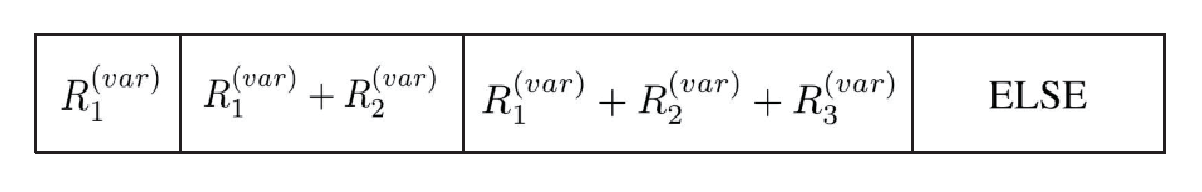
\includegraphics[width=\linewidth]{fig/mainwork/Roulette}
	%	\caption{Sensitive parameter selection by roulette method}
	%	\figlabel{fig:Roulette}
	%\end{figure}
\end{itemize}

通过计算熵方差选择最敏感参数,然后通过回归分析去得出最敏感参数的新值从而通过修改控制参数改变蛇形机器人运动步态实现环境的适应性运动。

\subsection{最敏感参数值的赋值}
在本文中,我们采用加权回归分析方法计算需要修改的最敏感步态参数的值,其中使用了梯度下降法求解拟合回归函数中的加权最小二乘问题。

\begin{itemize}
	\item 步骤一:列出拟合估计函数(式(\ref{fitfunction}))
	%fitting and estimation function
	\begin{eqnarray}\label{fitfunction}
	F_{w}(P_{t})=W^{T}P_{t}\,,&W=\begin{bmatrix}w_{1}\\ w_{2}\\ \vdots \\ w_{m}\end{bmatrix}
	\end{eqnarray}
	
	在式(\ref{fitfunction})中, $W$是拟合函数的系数矢量,$m$是系数的个数。$P_{t}$ 是实时采集到的蛇形机器人的关节角度,加速度和控制参数的实时值的数据矢量。然后我们可以得到误差函数(式(\ref{estimate})) ,误差函数采用平方和误差,$n$是矢量$\bm{P_{a}}$中的数据数量(即$\bm{P_{a}}$的维度减去控制参数的数量)。$\bm{Q}$是 $P_{i}$中的最敏感参数的数据矢量。
	%Square sum as an estimation
	\begin{eqnarray}\label{estimate}
	D(W)=\frac{1}{2n}(F_{w}(\bm{P_{a}})^{T}-\bm{Q})^{T}(F_{w}(\bm{P_{a}})^{T}-\bm{Q})
	\end{eqnarray}
	\begin{eqnarray}
	\bm{P_{a}}=\begin{bmatrix}P_{a,1}&P_{a,2}  &\cdots  &P_{a,n} \end{bmatrix}
	\end{eqnarray}
	\begin{eqnarray}
	\bm{Q}=\begin{bmatrix}Q_{a,1}& Q_{a,2}& \cdots & Q_{a,n}\end{bmatrix}^{T}
	\end{eqnarray}
	
	通过使误差函数$D(w)$最小化来得到拟合度最好的系数序列$W$,根据梯度下降算法原理,我们通过式(\ref{estimate})求导得到了式(\ref{Gradde})。
	%Gradient descent
	\begin{eqnarray}\label{Gradde}
	\nabla_{w}D=\frac{1}{n}\bm{P_{a}}(F_{w}(\bm{P_{a}})^{T}-\bm{Q})
	\end{eqnarray}
	
	\item 步骤二: 为了保证优势数据矢量拟合和加速回归,对优势数据矢量矩阵$\bm{P_{a}}$根据其对应的加速度采取加权操作(式(\ref{WEI},\ref{WeiGradde}))。
	%weighted gradient
	\begin{eqnarray}\label{WEI}
	\nabla_{w}D=\frac{1}{n}\bm{P_{a}}M(F_{w}(\bm{P_{a}})^{T}-\bm{Q})
	\end{eqnarray}
	\begin{eqnarray}\label{WeiGradde}
	M=\begin{bmatrix}
	\frac{a_{z,1}}{L_{s}}&0&\cdots&0\\
	0&\frac{a_{z,2}}{L_{s}}&\ddots&0\\
	\vdots&\ddots&\ddots&0\\
	0&\cdots&0&\frac{a_{z,n}}{L_{s}}
	\end{bmatrix}
	\end{eqnarray}
	在式(\ref{WeiGradde})中,$L_s$是可变学习步长,$M$是学习率矩阵。
	
	\item 步骤三:拟合系数矢量$W$(式(\ref{fit}))。
	%fitting the parameters
	\begin{eqnarray}\label{fit}
	W=W-\nabla_{w}D
	\end{eqnarray}
	在这一步中系数向量$W$被更新了。
	
	\item 步骤四:不断迭代以上步骤直到我们获取最拟合的系数向量。$W$的值最终趋于稳定状态。
\end{itemize}

迭代终止的时候,可以得到最优拟合系数向量$W_{best}$。通过将$W_{best}$代入式(\ref{result}),我们可以求解得到最敏感参数的回归结果。最终将结果用于步态的控制中,对于其他参数我们保留其原来的值,只修改最敏感参数的值。
%compensation result
\begin{eqnarray}\label{result}
Q_{t} = F_{w}(P_{t})=W^{T}P_{t}
\end{eqnarray}